
\section{Attenuation of sound waves}
\label{sec:sound_waves_att}

This section contains a simple discussion of the role of viscosity in
the attenuation of sound waves. Original work is by Stokes, 1845.

Let us start with the Navier-Stokes momentum equation, which will be
linearized by disregarding high-order deviations from equilibrium
values. The two viscosity coefficients always multiply the velocity
terms. Therefore, they are at to be taken at their equilibrium values,
since any departure would entail higher order terms. This points out
\ref{eq:NS_const_viscs} as our starting point. After linearizing, the
two equations are continuity and momentum.
\begin{align}
  & \frac{\partial\rho' }{\partial t}  + \rho_0 \divu =0 \\
  & \label{eq:NS_Newtonian_const_visc}
    \rho_0 \frac{\partial \bfu }{\partial t} =
    - c^2 \nabla \rho' + \mu \nabla^2 \bfu
    + ( \mu + \lambda ) \nabla\cdot ( \divu ) .
\end{align}
The same assumptions as those in
Eqs. \ref{eq:sound_small_u}-\ref{eq:sound_small_p} have been made.
Also, we write $\kappa = c^2$ for the proportinality of pressure
modulations with density modulations, where $c$ is the sound speed
when viscosity is neglected. The subscript ``$_0$'' is not written for
the viscosity coefficients for simplicity.

Eq. \ref{eq:NS_Newtonian_const_visc} may seem different from previous
expressions, but it is the correct one when $\mu$ is constant, but
incompressibility does not hold. In this case, the term in
\ref{eq:epsilon_term_with_divergence} is not zero, but rather gives
rise to a $\mu \nabla\cdot ( \divu )$ term.

Our systems is not as simple as the one in Section
\ref{sec:sound_waves}, where the continuity and momentum equations
where equally simple. There, we could easily eliminate either the
velocity or the density from our equations in order to get a single
equation for the other field. Now, the continuity equation is the
same, but the one for momentum one is much more involved. This leaves
us with eliminating the density as the only viable scheme.

If we apply the gradient operator to continuity, and differentiate
with respect to space in momentum, we arrive to this equation for
the velocity only:
\begin{equation}
  \label{eq:sound_att_Fourier}
  \frac{\partial^2 }{\partial t^2 } \mathbf{u} =
  c^2\nabla^2 \bfu + \nu \nabla^2\frac{\partial\bfu}{\partial t} +
  \zeta \nabla (\nabla\cdot \frac{\partial\bfu}{\partial t} ) ,
\end{equation}
where $\nu=\mu/\rho_0$, the usual kinematic viscosity, and we define
an additional kinematic bulk viscosity $\zeta=(\mu+\lambda)/\rho_0$.

Clearly, this reduces to our previous sound wave equation if there was
no viscosity.

Let us try a harmonic wave solution of the form
\begin{equation}
  \label{eq:wave_form_visc}
  \bfu = \Re\left[ \bfu_0 e^{i( \beta x - \omega t)} \right].
\end{equation}
Now $\bfu_0$ is a fixed amplitude vector, which may be parallel to
$\bhe$ in a longitudinal sound wave, but may also be perpendicular to
it, for a traverse wave. In general, of course, a wave may be a
combination of both.

Notice the usage of complex exponentials, which is common in wave
physics. Of course, the actual solution is real, so usually the real
part of the complex solution is kept (sometimes it is the imaginary,
which is equally valid). The flexibility comes partly from the fact
that $\mathbf{u}_0$ could be complex, which would represent a phase.
In our case, this is not important, but rather the possibility that
$\beta$ may be complex. In this case, its values encapsulates both a
real wave number and an spatial decay. Indeed, if
\[
  \beta = k + \alpha i ,
\]
then
\[
  \bfu = \bfu_0e^{- \alpha x} e^{i(k x - \omega t )} ,
\]
which clearly identifies $ \omega=2\pi /\lambda$ as the (real)
wave-number for a wave-lenght $ \lambda$, and $ \alpha=1 /\ell $, as a
sound attenuation coefficient, with $ \ell $ the attenuation length.
\index{sound attenuation coefficient}
\index{attenuation length}

Now, the time derivative is
\[
  \frac{\partial \bfu  }{\partial t }  = -i \omega \bfu ,
\]
and the second derivative,
\[
  \frac{\partial^2 \bfu   }{\partial t^2 }  = -\omega^2 \bfu.
\]

But, it is quite interesting that the two second space derivatives are
not the same. The Laplacian is
\[
\nabla^2 \bfu = -\beta^2 \bfu,
\]
while the gradient of the divergence is
\[
\nabla (\nabla\cdot \bfu ) = -\beta^2 u_{0x} \bhe_x.
\]
%
The latter then acts only on longitudinal waves: tranverse wave are
inherently divergence-free, since depend on one coordinate but point
toward a perpendicular direction (as in Couette and Poiseuille flows).
Let us consider them separately.

\subsection{Longitudinal waves}

In this case, insertion of the wave form \ref{eq:wave_form_visc} into
Eq. \ref{eq:NS_Newtonian_const_visc} yields

\begin{equation}
  -\omega^2 = - c^2\beta^2 + i (\nu+\zeta)  \omega \beta^2 .
\end{equation}
The expression includes both the shear and the volume bulk viscosity,
as seems fitting for a longitudinal disturbance, which involves
compression. If viscosities are negligible, the solution is just
\[
\omega =  c \beta ,
\]
%
the usual dispersion relation for sound of
Sec. \ref{sec:sound_waves}. In general, though:
\begin{equation}
  \label{eq:waves_att_dispersion}
  \beta^2 =
  \frac{\omega^2}{c^2 - i(\nu+\zeta)\omega}=
  \frac{\omega^2}{c^2}\frac{1}{1 -  i\omega/\omega_c},
\end{equation}
where we define the crossover angular frequency \index{crossover
  angular frequency}
\[
\omega_c := \frac{c^2}{\nu + \zeta }.
\]

This is the frequency above which the viscosity begins to be relevant.
Numerical values can be found in Table \ref{tbl:sound_att}. The
frequency is really high for the human hearing range, which goes up to
about $\SI{20}{\kilo\hertz}$ for humans. The record in the animal
kingdom is held by porpoises (\ref{fig:porpoise}), but it is only
about $\SI{160}{\kilo\hertz}$. Ultrasonic cleaners used in dentistry
operate at $\SI{40}{\kilo\hertz}$. Medical ultrasound for imaging goes
as high as $\SI{16}{\mega\hertz}$. Only acoustic microscopy
\cite{kp:AM} reaches a few \si{\giga\hertz}, matching our estimate for
air.


\begin{figure}
  \begin{center}
    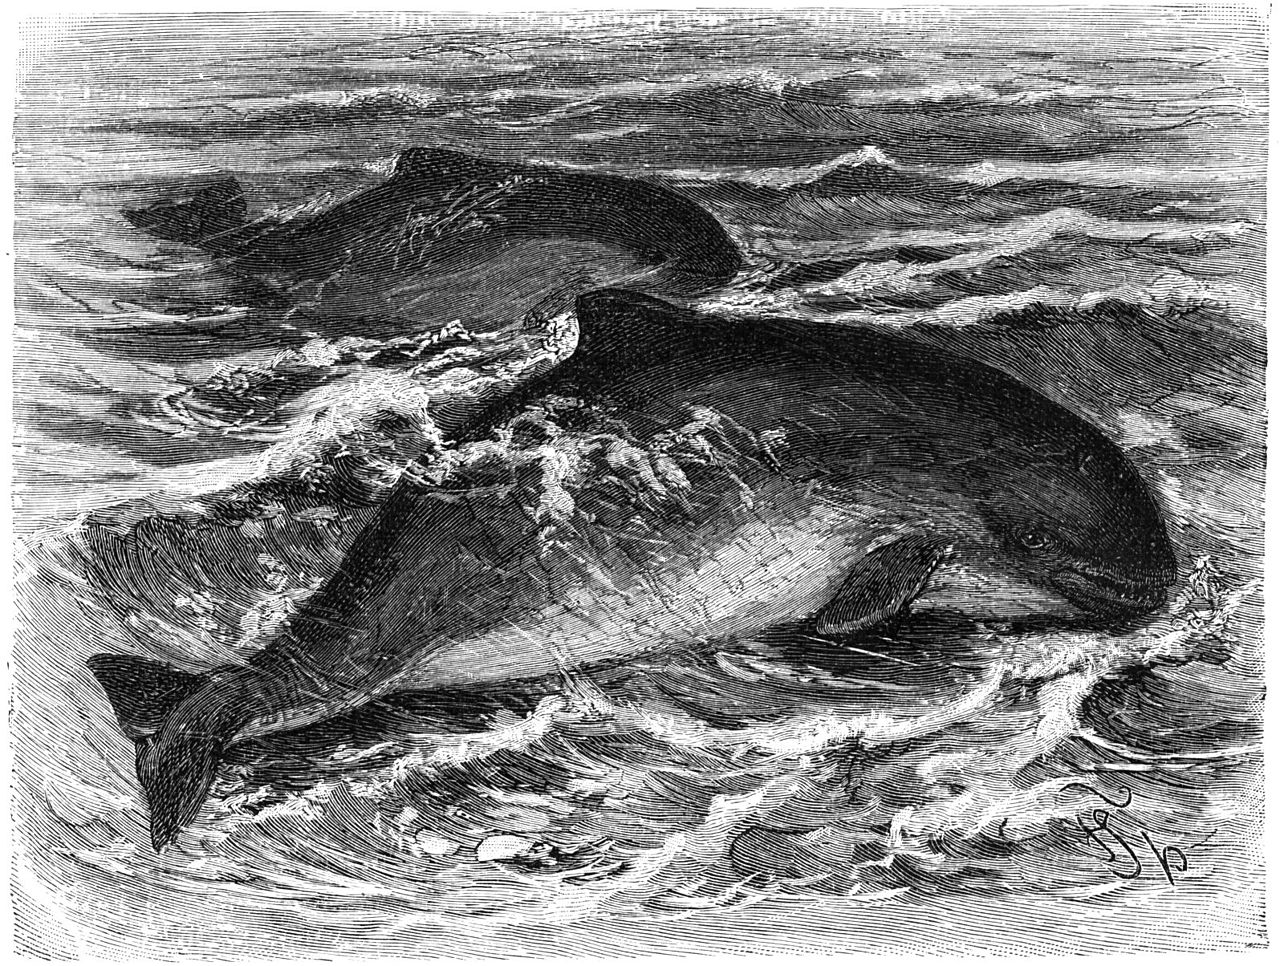
\includegraphics[width=0.7\textwidth]{figures/porpoises}
  \end{center}
  \caption{Harbor porpoises. From \cite{Brehms_Tierleben}.  \label{fig:porpoises}}
\end{figure}


\begin{table}
\begin{tabular}{|c|c|c|c|c|}
  \hline
    & $ c$ (m/s) &  $ \nu$ (m$^2$/s) & $\zeta$ (m$^2$/s) & $ f_c$ (GHz)\\
  \hline
  \hline
  water & $1480$& $ 1.0 \times 10^{-6}$ & $ 3.1 \times 10^{-6}$ & $79$ \\
  \hline
  air & $340$   & $ 1.48\times 10^{-5}$ & $ 5 \times 10^{-6}$ ? & $0.7$ \\
  \hline
\end{tabular}
\caption{Numerical values for two important substances. Values with
  question marks are speculative, since in Cramer\cite{Cramer} air is
  said to have a negligible bulk viscosity\ldots but in a graph this
  quantity's value is seen to be about half the shear viscosity value,
  and air is mostly nitrogen.
 \label{tbl:sound_att}}
\end{table}


\subsubsection{Low frequencies}


At frequencies much below the crossover frequency, we may expand the
term in the denominator in a Taylor series, then again for the square
root. The end result is
\[
\beta = \frac{\omega}{c} \left(1 + i   \frac{\omega}{2 \omega_c}\right).
\]
%
Therefore, the wave number is
\[
\beta = \frac{\omega}{c},
\]
as if there were no viscosity.

The attenuation coefficient is
\[ \alpha = \frac{\omega^2}{2 c\omega_c}=
\frac{\omega^2}{2 c^3}(\nu+\zeta). \]
%
It therefore grows as the square of the frequency.  This agrees is
called ``Stokes' law of sound'' \index{Stokes' law of sound}. Notice
that the alternative form is often found \cite{kp:SloS}
\[
  \alpha =  \frac{\omega^2}{\rho_0 c^3}((2/3) \mu+\eta /2 ),
\]
with $\eta= (2/3) \mu + \lambda$ the volume compressiblity.

This means that for that the highest sound in a porpoise's range, at
$\SI{160}{\kilo\hertz}$ the attenuation length would be about
$\SI{1.5}{\kilo\meter}$ (in water, of course). This may be important
for the long-range communication of these animals. For medical
ultrasound at $\SI{16}{\mega\hertz}$ this length is
$\SI{14}{\centi\meter}$, with water values (a fair approximation for
the human body.) This can have an impact for human tissues, in the
sense that in a distance of some tens of centimeters the energy of the
ultrasound waves is dissipated inside the body of the patient, and may
cause unwanted heating.

\subsubsection{High frequencies}

At frequencies much higher than the crossover, we may neglect the
``1'' in the denominator of \ref{eq:waves_att_dispersion}, to obtain
\[
\beta^2 = \frac{i \omega\omega_c}{c^2} .
\]
If we substitute the crossover frequency:
\[
\beta^2 = \frac{\omega}{i(\nu+\zeta)} =\frac{i \omega}{\nu+\zeta} 
\]
Recalling $i = e^{(pi/2)i} $, the solution is
\[
\beta =\sqrt{ \frac{\omega}{ \nu + \zeta }} e^{(\pi/4)i}.
\]

Therefore
\[
k=\alpha =\sqrt{\frac{\omega}{ 2 (\nu+ \zeta}}.
\]

This is an interesting result, since the attenuation coefficient is
equal to the wave number. The attenuation length is
\[
\ell= \frac{1}{\alpha}=\sqrt{\frac{ 2 (\nu+ \zeta)}{\omega}}
\]
The function looks therefore like a simple function
\[
g(x)= f(x/\ell) \qquad  f(x) = e^{-x}\cos(x) .
\]
In Figure \ref{fig:expcos}, it is seen to decay very fast, with just
one maximum of minimum of importance.



\subsubsection{At the crossover frequency}


A fast check on the above approximations is to see what happens when
the frequency is exactly the crossover frequency. At this point, the
growth of the attenuation coefficient as the square of frequency
crosses over to a growth as the square root. This would mean a bend in
a log-log plot, between two straight lines with different slopes. This
is shown in Figure \ref{fig:loglog}.

The extrapolation of the low frequency expression yields
\[
\alpha_c\approx \frac{\omega_c}{2 c} ,
\]

whereas the high frequency expression yields
\[
\alpha_c\approx \frac{\omega_c}{\sqrt{2} c} ,
\]
which are similar.

The exact expression can be shown to be, after some involved algebra,
\[
\alpha_c =\frac{ \sin(\pi/8) \omega_c }{ (2^{1/4} c } ,
\]
a value just a bit below the other two. This means the approximations
remain quite fair up to the limit of their respective ranges.

By the way, for water this value corresponds to an attenuation length
of about \SI{58}{\nano\meter}, which is really short. For air, it is
about \SI{1.5}{\micro\meter}, the size of a really small cell.


\subsection{Transverse waves}

We tend to think, sound waves are longitudinal. We here discuss how
they may have a transverse component, but it is dampened at al
frequencies.

If we write Eq. \ref{eq:sound_att_Fourier} for the $y$ or $z$
Cartesian component, we find
\[
-\omega^2 =  i \nu \omega \beta^2 ,
\]
or
\[
\beta^2 = \frac{i \omega}{\nu}.
\]
Only $\nu$ is involved, which is fitting: transverse waves involve
only shear, not compression.

The expression is very similar to the one for longitudinal waves at
high frequencies, only this one is valid at \emph{all} frequencies.
Its solution is
\[
k = \alpha = \sqrt{ \frac{\omega}{ 2 \nu}}.
\]
Figure \ref{fig:expcos} still applies to these waves, with the
difference that the decay length is
\[
\ell= \frac{1}{\alpha}=\sqrt{\frac{ 2 \nu}{\omega}}
\]

For frequencies of ordinary ``sound'', i.e. audible frequencies, that
length is quite small. With the numerical data in the Table, that
length is only about \SI{0.7}{\milli\meter} for aire, at a very low
frequency of \SI{10}{\hertz} (just below the lower hearing threshold),
and will decrease further as the inverse of the square root of the
frequency.




